% !TEX root = ../main.tex
% ============================================================================
% Results
% ============================================================================
\chapter{Results}
\label{ch:results}

This chapter reports the experimental results. It first establishes the
from-scratch capacity baselines that quantify the accuracy cost of shrinking HiVT
(Section~\ref{sec:res_baselines}) and the recipe choices that make those baselines
honest (Section~\ref{sec:res_recipe}). It then presents the central result---the
contrast between the two distillation objectives on HiVT-32
(Section~\ref{sec:res_kd32})---and its replication, with a larger relative gain, on
the smaller HiVT-16 (Section~\ref{sec:res_kd16}). Finally it consolidates the
accuracy--capacity trade-off across all models (Section~\ref{sec:res_frontier}),
measures the inference efficiency that motivates the whole exercise
(Section~\ref{sec:res_eff}), and closes with qualitative and diagnostic analysis
(Section~\ref{sec:res_qual}). Unless noted otherwise, every number is computed by
\texttt{eval.py} on the full Argoverse~1 validation split, and the primary metric
is minFDE$_6$.

\section{From-Scratch Capacity Baselines}
\label{sec:res_baselines}

Table~\ref{tab:baselines} reports the four HiVT widths trained (or, for the
authors' released checkpoints, evaluated) without any distillation. They span a
$55\times$ range in parameters and form the reference frame for every later claim:
the distillation gain is always measured as movement \emph{relative to the
same-width from-scratch model}.

\begin{table}[htbp]
  \centering
  \caption{From-scratch capacity baselines on the Argoverse~1 validation split.
    HiVT-128 and HiVT-64 are the authors' released checkpoints; HiVT-32 and
    HiVT-16 are trained in this work under the recipe of
    Section~\ref{sec:res_recipe}. Lower is better for all columns. HiVT-16 uses
    $2$ attention heads (Section~\ref{ssec:res_heads}).}
  \label{tab:baselines}
  \begin{tabular}{lrrrrrr}
    \toprule
    Model & Params & minADE & minFDE & MR & mixNLL & calib.\ err \\
    \midrule
    HiVT-128 (teacher) & 2{,}559{,}993 & 0.6611 & 0.9692 & 0.0920 & 21.05 & 0.0466 \\
    HiVT-64            & 653{,}369    & 0.6869 & 1.0301 & 0.1026 & 23.02 & 0.0416 \\
    HiVT-32            & 170{,}073    & 0.7361 & 1.1574 & 0.1217 & 26.61 & 0.0325 \\
    HiVT-16            & 45{,}929     & 0.8858 & 1.6053 & 0.1988 & 35.22 & 0.0279 \\
    \bottomrule
  \end{tabular}
\end{table}

Two patterns matter for what follows. First, geometric error grows
\emph{faster than linearly} as width falls: halving width from $64$ to $32$ costs
$+0.127$\,m minFDE, but halving again from $32$ to $16$ costs $+0.448$\,m---the
small end of the ladder is where capacity hurts most, and therefore where
distillation has the most to recover. Second, the from-scratch models are already
\emph{well calibrated} (calibration error $\le 0.047$ everywhere, in fact lowest at
the smallest widths): calibration is not a pre-existing defect to be fixed, which
is precisely why a distillation method that \emph{damages} it (v1,
Section~\ref{sec:res_kd32}) is unacceptable even when it improves geometry.

\section{Student Recipe Selection}
\label{sec:res_recipe}

The students trained in this work require two width-dependent choices---learning
rate and attention-head count---that were fixed by short sweeps before any
distillation. Settling these on the \emph{from-scratch} model ensures the later
distillation comparison is against a properly tuned, not a handicapped, baseline.

\subsection{Learning rate}
\label{ssec:res_lr}
HiVT-32 trains best at $\eta=3\times10^{-3}$, selected by a learning-rate sweep on
a $25\%$-data proxy (logged to Weights \& Biases). HiVT-16, in contrast,
\emph{diverges in quality} at that rate: Table~\ref{tab:lr16} shows the $25\%$
proxy sweep, in which $\eta=1\times10^{-3}$ is best by a wide margin and the higher
rates ($2$--$3\times10^{-3}$) nearly double minFDE. The same $\eta=3\times10^{-3}$
that is optimal for HiVT-32 drives HiVT-16 to minFDE $3.22$ on full data---a
non-converged model. The smaller network thus needs the gentler step; this
$\eta=1\times10^{-3}$ is used for all HiVT-16 runs.

\begin{table}[htbp]
  \centering
  \caption{HiVT-16 learning-rate sweep ($25\%$ data, short schedule). $\eta=1\times
    10^{-3}$ is best on every metric. Lower is better.}
  \label{tab:lr16}
  \begin{tabular}{lrrrr}
    \toprule
    Metric & $\eta=5\mathrm{e}{-}4$ & $\eta=1\mathrm{e}{-}3$ & $\eta=2\mathrm{e}{-}3$ & $\eta=3\mathrm{e}{-}3$ \\
    \midrule
    minADE     & 3.6572 & \textbf{1.5074} & 1.7749 & 1.7232 \\
    minFDE     & 9.4680 & \textbf{2.9142} & 3.4486 & 3.3241 \\
    MR         & 0.7684 & \textbf{0.3186} & 0.4868 & 0.4748 \\
    calib.\ err& 0.0860 & \textbf{0.0284} & 0.0729 & 0.0717 \\
    mixNLL     & 92.76  & \textbf{53.20}  & 69.36  & 67.55  \\
    \bottomrule
  \end{tabular}
\end{table}

\subsection{Attention heads}
\label{ssec:res_heads}
HiVT uses $8$ attention heads by default, so the per-head dimension shrinks with
width (Section~\ref{ssec:setup_models}). At HiVT-32 this is benign:
Table~\ref{tab:heads32} compares $2$ heads (head dimension $16$) against the
default $8$ (head dimension $4$) on the from-scratch model, and the two are
indistinguishable on geometry---every displacement metric moves under $1.5\%$ and
the differences flip sign, i.e.\ single-run noise. At $d{=}32$ there is simply not
enough width for $8$ heads to express more than $2$, so head count is not a
meaningful lever and the baseline may use either; the default $8$ is retained.

\begin{table}[htbp]
  \centering
  \caption{HiVT-32, $2$ vs.\ $8$ attention heads, from-scratch (no KD), full data.
    Only \texttt{num\_heads} differs. Geometry is a tie; calibration differs only
    within plausible single-run variance.}
  \label{tab:heads32}
  \begin{tabular}{lrrr}
    \toprule
    Metric & 2 heads & 8 heads & $\Delta$ \\
    \midrule
    minADE      & 0.7381 & 0.7365 & $+0.22\%$ \\
    minFDE      & 1.1622 & 1.1574 & $+0.41\%$ \\
    MR          & 0.1242 & 0.1225 & $+1.40\%$ \\
    mixNLL      & 26.891 & 26.695 & $+0.73\%$ \\
    calib.\ err & 0.0316 & 0.0362 & $-12.8\%$ \\
    \bottomrule
  \end{tabular}
\end{table}

HiVT-16 is the opposite case. The per-head dimension is $16/\mathrm{nh}$, so the
default $8$ heads leave only $2$ channels per head---too few for the attention to
be expressive. Table~\ref{tab:heads16} sweeps nh $\in\{2,4,8\}$ on the $25\%$
proxy: geometry degrades \emph{monotonically} as the head dimension shrinks, with
minFDE rising from $2.95$ (nh$=2$, head dimension $8$) through $3.25$ (nh$=4$) to
$3.69$ (nh$=8$, head dimension $2$)---a $25\%$ relative loss---and the best-mode
regression NLL nearly doubling at nh$=8$, a sign the smallest-head model trains
poorly. Two heads is clearly best, so HiVT-16 uses $2$ heads for every reported
result. This mirrors and sharpens the HiVT-32 finding: head count is immaterial
when the width is ample (HiVT-32) but becomes a real lever once the width is small
enough that adding heads starves each of dimension (HiVT-16).

\begin{table}[htbp]
  \centering
  \caption{HiVT-16 attention-head sweep ($25\%$ data proxy, from-scratch, no KD;
    final-epoch validation, minFDE confirmed by best-checkpoint selection). The
    per-head dimension is $16/\mathrm{nh}$. Geometry worsens monotonically as heads
    are added and each is starved of dimension; $2$ heads is best. Lower is better.}
  \label{tab:heads16}
  \begin{tabular}{lrrr}
    \toprule
    Metric & nh${=}2$ (dim 8) & nh${=}4$ (dim 4) & nh${=}8$ (dim 2) \\
    \midrule
    minADE        & \textbf{1.50} & 1.53 & 1.87 \\
    minFDE        & \textbf{2.95} & 3.25 & 3.69 \\
    MR            & \textbf{0.338} & 0.394 & 0.505 \\
    brier-minFDE  & \textbf{3.58} & 3.87 & 4.33 \\
    reg-loss      & 0.144 & 0.142 & 0.284 \\
    \bottomrule
  \end{tabular}
\end{table}

\section{Distillation on HiVT-32: Mean-Target vs.\ Distribution-Matching}
\label{sec:res_kd32}

This section is the core empirical result. It shows, on HiVT-32, that the naive
mean-target objective (v1) improves geometry but \emph{collapses calibration},
that the failure is the per-mode scale shrinkage predicted in
Section~\ref{ssec:method_calib}, and that the distribution-matching objective (v2)
retains the full geometric gain while repairing calibration.

\subsection{The distillation-weight sweep}
\label{ssec:res_sweep32}
Figure~\ref{fig:lambda32} sweeps the distillation weight $\lambda$ for v1 on a
$25\%$-data proxy. The five panels tell the whole v1 story at once: geometry
(minFDE) improves sharply and then saturates, while every calibration diagnostic
moves the wrong way---mixNLL turns up, the mean Laplace scale $b$ \emph{shrinks}
monotonically, and the calibration error climbs steeply. Crucially the mode-weight
entropy is \emph{flat} across $\lambda$: the damage is not a collapse of the
mixture weights but a sharpening of each mode's predicted spread, exactly the
signature derived analytically in Section~\ref{ssec:method_calib}. The proxy ranks
$\lambda\!\approx\!0.25$--$0.5$ best on geometry; $\lambda=0.5$ is carried forward
as the operating point, being the standard value in the distillation literature
and a reasonable geometry/calibration compromise.

\begin{figure}[htbp]
  \centering
  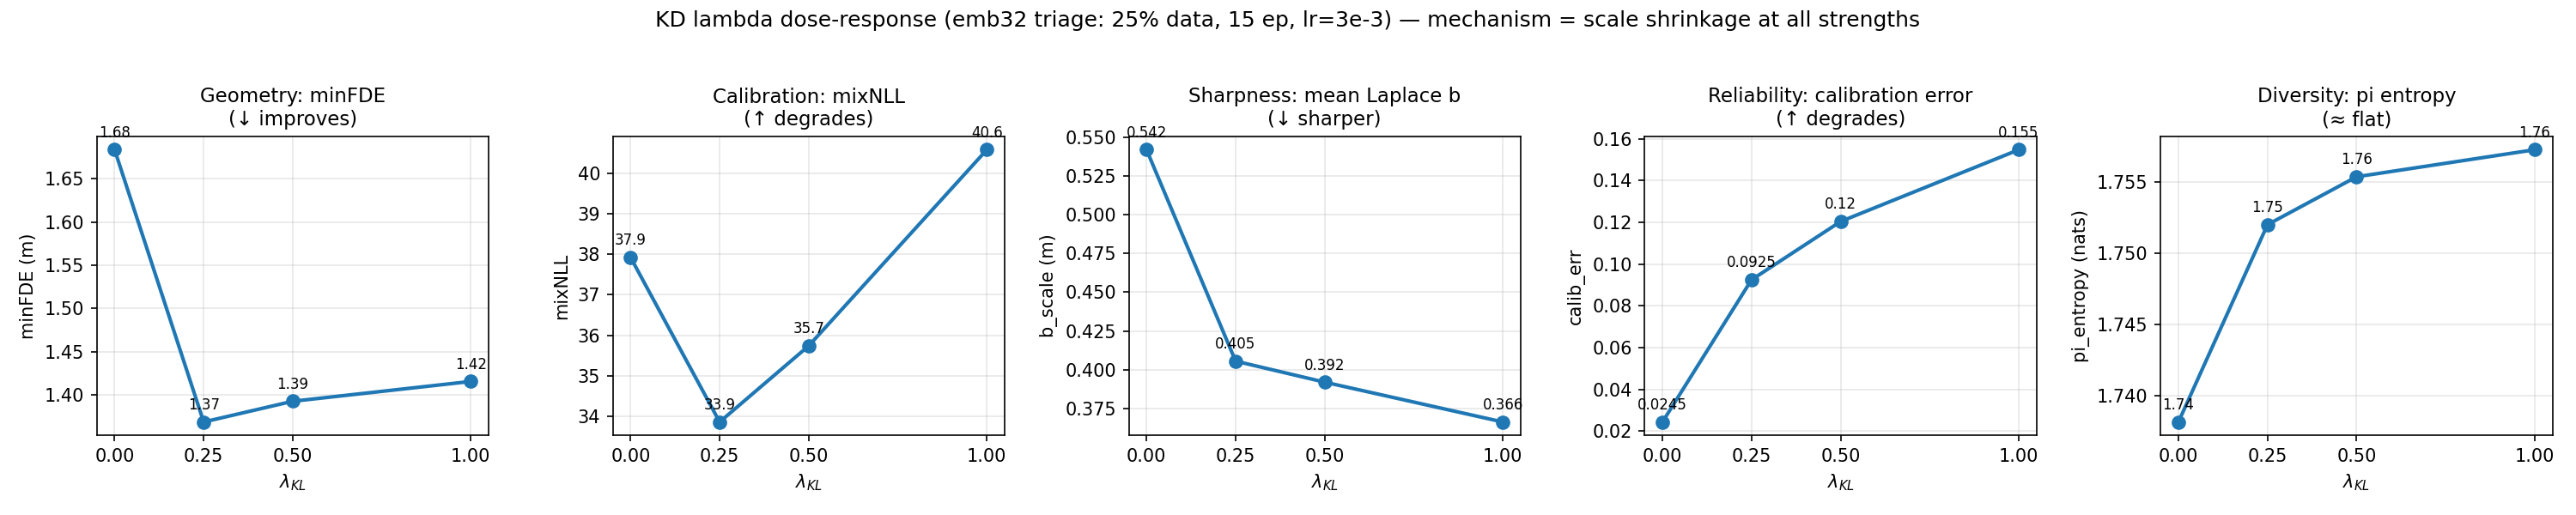
\includegraphics[width=\linewidth]{figures/kd_lambda_sweep.png}
  \caption{HiVT-32 v1 (mean-target) distillation-weight sweep ($25\%$ data).
    Geometry (minFDE, left) improves with $\lambda$, but mixNLL, calibration
    error rise and the mean Laplace scale $b$ shrinks, while mode-weight entropy
    (right) is unchanged. The pathology is scale shrinkage, not mode collapse.}
  \label{fig:lambda32}
\end{figure}

\subsection{v1: accuracy up, calibration down}
\label{ssec:res_v1}
Table~\ref{tab:ab32} is the clean A/B at full data and the chosen $\lambda=0.5$:
the same recipe, with the distillation term switched on. Geometry improves
substantially and consistently---minFDE $-9.2\%$, MR $-13.8\%$, minADE
$-5.5\%$---and the official ranking metric brier-minFDE improves by $5.3\%$. But
the full-distribution metrics collapse: mixNLL worsens by $41\%$ and the
calibration error rises five-fold, from $0.036$ to $0.183$. The mean scale $b$
drops $35\%$ ($0.413\to0.268$): the student has been driven well below its own
calibrated width and is now systematically over-confident, as the reliability
curves of Figure~\ref{fig:reliability} confirm---the predicted intervals cover far
fewer ground-truth points than their nominal probability, and the under-coverage
worsens monotonically with $\lambda$. The same shrinkage shows in the two final
rows: the predicted $90\%$ interval now captures only $71.3\%$ of ground-truth
endpoints (cov@p90 $0.900\to0.713$), and even HiVT's own winner-takes-all
regression NLL (reg-loss) worsens ($-0.246\to-0.188$)---the single \emph{best} mode
assigns lower density to the truth despite sitting geometrically closer to it,
because its scale has shrunk faster than its location error has fallen. The
over-confidence is thus visible even on the best mode, not only across the full
mixture.

\begin{table}[htbp]
  \centering
  \caption{HiVT-32, v1 distillation A/B (full data): no KD ($\lambda{=}0$) vs.\
    mean-target KD ($\lambda{=}0.5$). v1 trades calibration for geometry. Lower is
    better for all rows except $b$-scale (the drop reflects over-confidence),
    cov@p90 (closer to the nominal $0.90$ is better, so the fall to $0.713$ is
    under-coverage), and reg-loss (more negative is better, so the rise is worse).}
  \label{tab:ab32}
  \begin{tabular}{lrrr}
    \toprule
    Metric & no KD & v1 ($\lambda{=}0.5$) & $\Delta$ \\
    \midrule
    minADE        & 0.7365 & 0.6958 & $-5.5\%$ \\
    minFDE        & 1.1574 & 1.0509 & $-9.2\%$ \\
    MR            & 0.1225 & 0.1056 & $-13.8\%$ \\
    brier-minFDE  & 1.8197 & 1.7235 & $-5.3\%$ \\
    mixNLL        & 26.695 & 37.624 & $+40.9\%$ \\
    calib.\ err   & 0.0362 & 0.1827 & $+405\%$ \\
    $b$-scale     & 0.4129 & 0.2678 & $-35.1\%$ \\
    cov@p90       & 0.900  & 0.713  & $-0.187$ \\
    reg-loss      & $-0.2459$ & $-0.1876$ & $+0.058$ \\
    \bottomrule
  \end{tabular}
\end{table}

\begin{figure}[htbp]
  \centering
  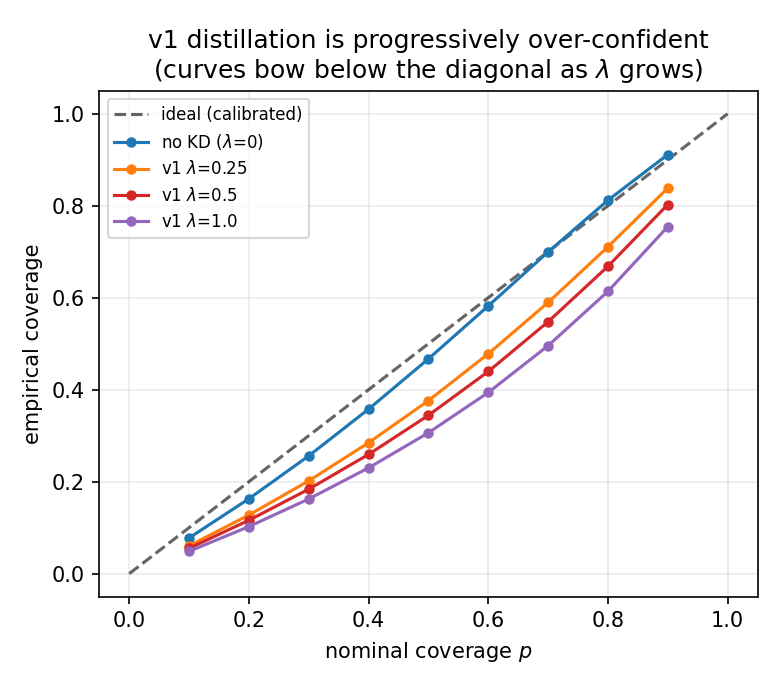
\includegraphics[width=0.62\linewidth]{figures/reliability_v1_sweep.png}
  \caption{Reliability (empirical vs.\ nominal coverage) for HiVT-32 under v1
    distillation. The no-KD model tracks the diagonal; as $\lambda$ grows the
    curves bow progressively below it, i.e.\ the predicted intervals are too narrow
    (over-confident). Coverage data from the $\lambda$-sweep of
    Figure~\ref{fig:lambda32}.}
  \label{fig:reliability}
\end{figure}

This is the negative result that motivates v2, summarised as: \emph{mean-target
mixture distillation improves geometric accuracy and the official Argoverse ranking
metric but degrades full-distribution calibration, because it transfers the
teacher's mode locations and weights while discarding its predictive variance,
producing over-confident student mixtures.}

\subsection{v2: accuracy retained, calibration repaired}
\label{ssec:res_v2}
The distribution-matching objective scores Monte-Carlo samples drawn with the
teacher's own scales, so collapsing the student's scales no longer minimises the
loss. Table~\ref{tab:v2_32} places v2 beside v1 and the baseline.

\begin{table}[htbp]
  \centering
  \caption{HiVT-32: distribution-matching (v2) vs.\ mean-target (v1) vs.\ no KD,
    full data, $\lambda{=}0.5$. v2 matches v1's geometry and repairs its
    calibration, ending up better calibrated than the from-scratch baseline and the
    teacher. Lower is better except $b$-scale (closer to the calibrated $\approx
    0.41$ is better) and cov@p90 (closer to $0.90$ is better).}
  \label{tab:v2_32}
  \begin{tabular}{lrrrr}
    \toprule
    Metric & no KD & v1 & \textbf{v2} & teacher \\
    \midrule
    minADE       & 0.7365 & 0.6958 & \textbf{0.6982} & 0.6611 \\
    minFDE       & 1.1574 & 1.0509 & \textbf{1.0505} & 0.9692 \\
    MR           & 0.1225 & 0.1056 & \textbf{0.1063} & 0.0920 \\
    brier-minFDE & 1.8197 & 1.7235 & \textbf{1.7240} & --- \\
    mixNLL       & 26.69  & 37.62  & \textbf{24.18}  & 21.05 \\
    calib.\ err  & 0.0362 & 0.1827 & \textbf{0.0275} & 0.0466 \\
    $b$-scale    & 0.4129 & 0.2678 & \textbf{0.4126} & 0.358 \\
    cov@p90      & 0.900  & 0.713  & \textbf{0.909}  & 0.894 \\
    \bottomrule
  \end{tabular}
\end{table}

v2 ties v1 on geometry exactly (minFDE $1.0505$ vs.\ $1.0509$) and eliminates the
calibration penalty entirely: the calibration error falls to $0.0275$---$6.6\times$
better than v1, and lower than both the from-scratch baseline and the teacher---and
cov@p90 returns to nominal. The mean scale recovers to $0.413$, the student's own
calibrated width. (That this exceeds the teacher's $0.358$ is expected and correct:
a less-accurate student has larger typical error, so honest calibration
\emph{requires} a wider scale; v1's error was being sharper than even the teacher.)
v2 thus delivers the full accuracy gain of distillation at zero calibration cost,
confirming the chapter's central hypothesis on HiVT-32.

\section{Distillation on HiVT-16}
\label{sec:res_kd16}

The HiVT-16 experiments test whether the v2 result replicates at a smaller width
and whether, as hypothesised, the relative benefit \emph{grows} as the student
shrinks. Because the v1 calibration failure is already established, HiVT-16 is run
directly with v2.

\subsection{Distillation-weight sweep}
The $\lambda$-sweep ($25\%$ proxy, Table~\ref{tab:kl16}) shows a clear knee at
$\lambda=1.0$---higher than HiVT-32's optimum, consistent with a smaller student
benefiting from a stronger teacher signal. Geometry improves monotonically up to
$\lambda=1.0$ (minFDE $-16.4\%$ vs.\ no KD) and then regresses at $\lambda=2.0$.
Calibration stays intact throughout: mixNLL \emph{improves} with $\lambda$ and the
scale stays in the healthy band, with none of the v1 collapse.

\begin{table}[htbp]
  \centering
  \caption{HiVT-16 v2 distillation-weight sweep ($25\%$ data). Geometry bottoms at
    $\lambda{=}1.0$; calibration is preserved throughout. Best geometry per row in
    bold. Lower is better except $b$-scale (closer to $\approx 0.73$ better).}
  \label{tab:kl16}
  \begin{tabular}{lrrrr}
    \toprule
    Metric & $\lambda{=}0$ & $\lambda{=}0.5$ & $\boldsymbol{\lambda{=}1.0}$ & $\lambda{=}2.0$ \\
    \midrule
    minADE      & 1.3628 & 1.2701 & \textbf{1.1770} & 1.2400 \\
    minFDE      & 2.6471 & 2.4878 & \textbf{2.2125} & 2.3655 \\
    MR          & 0.2995 & 0.3024 & \textbf{0.2571} & 0.2632 \\
    calib.\ err & 0.0195 & 0.0259 & 0.0244 & 0.0291 \\
    $b$-scale   & 0.7334 & 0.6750 & 0.6958 & 0.6820 \\
    mixNLL      & 51.30  & 45.62  & 44.88  & 43.75 \\
    \bottomrule
  \end{tabular}
\end{table}

\subsection{Full-data confirmation}
The proxy winner ($\lambda=1.0$, v2) was retrained on full data for $64$ epochs and
A/B'd against the matched no-KD baseline (Table~\ref{tab:ab16}). The result is the
chapter's strongest: minFDE improves by $\mathbf{22.7\%}$ ($1.605\to1.240$) and MR
by $33\%$, \emph{exceeding} the proxy's $-16.4\%$ prediction---the KD benefit
compounded with full data and a full schedule rather than fading. And, unlike v1 at
HiVT-32, \emph{every} calibration metric moves the right way: mixNLL $-16.8\%$,
calibration error $-5.1\%$, cov@p90 stays nominal, and the scale stays healthy.
There is no calibration tax; the v2 objective delivers geometry and calibration
together, now confirmed at a second width.

\begin{table}[htbp]
  \centering
  \caption{HiVT-16, v2 distillation A/B (full data, $\lambda{=}1.0$): the same
    recipe with KD switched on. Both geometry and calibration improve. Lower is
    better for all rows except $b$-scale (both values are in the healthy band) and
    cov@p90 ($0.90$ is nominal).}
  \label{tab:ab16}
  \begin{tabular}{lrrr}
    \toprule
    Metric & no KD & v2 ($\lambda{=}1.0$) & $\Delta$ \\
    \midrule
    minADE       & 0.8858 & 0.7762 & $-12.4\%$ \\
    minFDE       & 1.6053 & 1.2402 & $-22.7\%$ \\
    MR           & 0.1988 & 0.1333 & $-32.9\%$ \\
    brier-minFDE & 2.2565 & 1.9147 & $-15.1\%$ \\
    mixNLL       & 35.22  & 29.32  & $-16.8\%$ \\
    calib.\ err  & 0.0279 & 0.0265 & $-5.1\%$ \\
    cov@p90      & 0.9064 & 0.9034 & $\approx$ nominal \\
    \bottomrule
  \end{tabular}
\end{table}

\paragraph{Smaller students benefit more.}
The relative geometric gain from v2 is $-22.7\%$ minFDE at HiVT-16 against $-9.2\%$
at HiVT-32---roughly $2.5\times$ larger for the smaller network. This is the
expected ordering: the student with the largest gap to the teacher has the most to
gain from its guidance, and distillation is correspondingly more valuable exactly
where capacity is scarcest.
% TODO(optional): if the second-seed HiVT-16 run (kl1.0-full-s1) is evaluated,
% report mean +/- spread here to harden the calibration claims.

\section{The Accuracy--Capacity Frontier}
\label{sec:res_frontier}

Table~\ref{tab:frontier} and Figure~\ref{fig:frontier} consolidate every model on
a single accuracy--capacity axis. The headline reading is that distillation moves
each student up roughly a full size-class at \emph{zero inference cost}.

\begin{table}[htbp]
  \centering
  \caption{All models on the accuracy--capacity frontier. KD students use v2
    distribution-matching. Lower is better. The KD students approach the next
    larger from-scratch model while keeping their own (much smaller) parameter
    count.}
  \label{tab:frontier}
  \begin{tabular}{lrrrrr}
    \toprule
    Model & Params & minADE & minFDE & MR & calib.\ err \\
    \midrule
    HiVT-16            & 45{,}929   & 0.8858 & 1.6053 & 0.1988 & 0.0279 \\
    \textbf{HiVT-16 KD v2} & 45{,}929 & \textbf{0.7762} & \textbf{1.2402} & \textbf{0.1333} & \textbf{0.0265} \\
    HiVT-32            & 170{,}073  & 0.7361 & 1.1574 & 0.1217 & 0.0325 \\
    \textbf{HiVT-32 KD v2} & 170{,}073 & \textbf{0.6982} & \textbf{1.0505} & \textbf{0.1063} & \textbf{0.0275} \\
    HiVT-64            & 653{,}369  & 0.6869 & 1.0301 & 0.1026 & 0.0416 \\
    HiVT-128 (teacher) & 2{,}559{,}993 & 0.6611 & 0.9692 & 0.0920 & 0.0466 \\
    \bottomrule
  \end{tabular}
\end{table}

\begin{figure}[htbp]
  \centering
  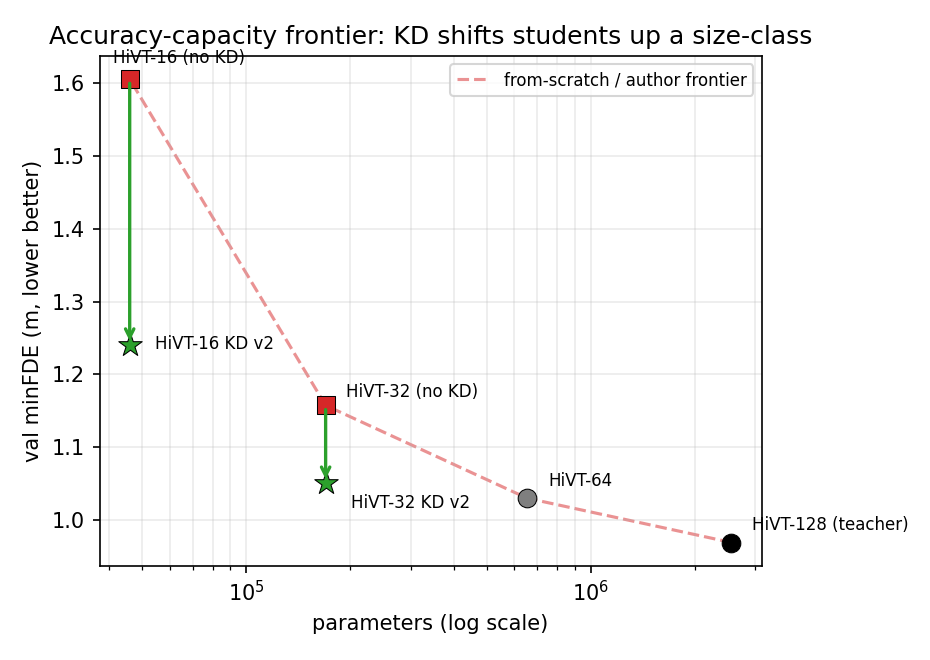
\includegraphics[width=0.78\linewidth]{figures/accuracy_capacity_frontier.png}
  \caption{Accuracy--capacity frontier (minFDE vs.\ parameters, log scale). The
    dashed line is the from-scratch frontier; green arrows show the effect of v2
    distillation. Each KD student is pulled down toward the next larger model's
    accuracy while retaining its own parameter count.}
  \label{fig:frontier}
\end{figure}

Quantitatively, HiVT-32 KD v2 (minFDE $1.0505$) lands essentially on top of the
from-scratch HiVT-64 ($1.0301$), a model with $3.8\times$ more parameters: it
recovers $\approx 84\%$ of the HiVT-32$\to$HiVT-64 gap, and $\approx 57\%$ of the
much larger HiVT-32$\to$HiVT-128 gap, at $6.6\%$ of the teacher's parameters.
HiVT-16 KD v2 (minFDE $1.2402$) reproduces the pattern one width down: it recovers
$\approx 81\%$ of the HiVT-16$\to$HiVT-32 gap, landing within $7.2\%$ of the
\emph{un-distilled} HiVT-32 while using only $27\%$ of its parameters. In both
cases distillation buys roughly a full size-class of accuracy for free, and---with
the v2 objective---without the calibration penalty that would otherwise make the
trade unusable downstream.

\section{Inference Efficiency}
\label{sec:res_eff}

The motivation for a smaller model is cheaper inference. The savings come on two
axes that behave very differently: parameters/memory, which scale cleanly with
width, and latency, which is sublinear and regime-dependent.

\paragraph{Parameters and memory.}
The parameter reduction is exact and unconditional: HiVT-32 and HiVT-16 use $6.6\%$
and $1.8\%$ of the teacher's parameters ($15\times$ and $55\times$ smaller). On GPU
this translates directly into peak memory (Table~\ref{tab:gpumem}): at batch size
$128$ the student-16 uses $543$\,MB against the teacher's $3410$\,MB---a $6.3\times$
reduction---and the ratio \emph{widens} with batch size. This is the clean,
reliable efficiency win: it permits larger batches, smaller GPUs, or co-locating
more models on one device.

\begin{table}[htbp]
  \centering
  \caption{Peak GPU memory (MB), RTX~5060, real validation batches. The memory
    saving scales with width and grows with batch size.}
  \label{tab:gpumem}
  \begin{tabular}{rrrrrr}
    \toprule
    Batch & HiVT-128 & HiVT-32 & HiVT-16 & T/S32 & T/S16 \\
    \midrule
    1   & 70.4   & 40.5  & 36.6  & 1.7$\times$ & 1.9$\times$ \\
    8   & 203.6  & 76.8  & 56.7  & 2.7$\times$ & 3.6$\times$ \\
    32  & 799.2  & 241.4 & 147.9 & 3.3$\times$ & 5.4$\times$ \\
    64  & 1519.3 & 435.7 & 257.0 & 3.5$\times$ & 5.9$\times$ \\
    128 & 3409.8 & 954.3 & 543.5 & 3.6$\times$ & \textbf{6.3$\times$} \\
    \bottomrule
  \end{tabular}
\end{table}

\paragraph{Latency.}
Latency tells a more nuanced story (Table~\ref{tab:latency}). On CPU the speedup is
far sublinear in the parameter reduction and depends strongly on batch size: at
$bs{=}1$ (true online inference) HiVT-32 is only $3.0\times$ faster despite $15\times$
fewer parameters, because a fixed $\approx 7$\,ms floor---graph construction, the
fixed transformer-layer count, PyG dispatch, memory-bound scatter/norm ops, all
\emph{independent} of embedding width---dominates the tiny $d^2$ matmuls. Batching
amortises that floor and widens the gap, to $5.5\times$ (HiVT-32) and $11.5\times$
(HiVT-16) around $bs{=}8$--$32$, after which limited CPU parallelism causes
per-scene latency to turn back up. On GPU the latency advantage nearly
vanishes ($\approx 1$--$2.6\times$, occasionally below $1\times$): the GPU has so
much parallelism that the students' small matmuls never saturate it, so the
width-independent overhead dominates and shrinking the model barely changes
wall-clock. The conclusion is that ``$55\times$ smaller'' is a memory claim, not a
speed claim: the unconditional dividend is memory, while the latency win is real
only on CPU under modest batching.

\begin{table}[htbp]
  \centering
  \caption{Per-scene inference latency (ms), median of $30$ passes. CPU:
    \texttt{OMP\_NUM\_THREADS=4}. GPU: RTX~5060 (read coarsely---the medians are
    heavy-tailed). ``speedup'' is teacher $\div$ student.}
  \label{tab:latency}
  \begin{tabular}{rrrrrrr}
    \toprule
    & \multicolumn{3}{c}{CPU latency (ms)} & \multicolumn{3}{c}{GPU latency (ms)} \\
    \cmidrule(lr){2-4}\cmidrule(lr){5-7}
    Batch & T-128 & S-32 & S-16 & T-128 & S-32 & S-16 \\
    \midrule
    1   & 20.82 & 6.86 & 6.11 & 46.84 & 43.64 & 26.14 \\
    8   & 16.07 & 2.95 & 2.14 & 10.37 & 9.02  & 6.89 \\
    32  & 27.05 & 4.68 & 2.35 & 4.02  & 2.68  & 3.08 \\
    64  & 27.85 & 5.85 & 2.87 & 3.44  & 1.85  & 1.30 \\
    128 & ---   & ---  & ---  & 1.54  & 1.56  & 1.42 \\
    \bottomrule
  \end{tabular}
\end{table}

A further practical point: at $bs{=}1$ the GPU is launch-bound and actually
\emph{slower} than the CPU ($26$--$47$\,ms vs.\ $6$--$21$\,ms), because thousands of
tiny kernel launches and host/device synchronisation dominate a single small graph.
For genuine online, one-scene-at-a-time deployment the distilled student is best run
on CPU; the GPU pays off only once inputs are batched.

\section{Qualitative and Diagnostic Analysis}
\label{sec:res_qual}

\paragraph{Predicted multimodality.}
Figure~\ref{fig:traj} shows the six predicted modes for a representative focal
agent at an intersection, ranked by probability, against the observed history and
ground truth. The model spreads probability over distinct, plausible
manoeuvres---differing in reach and curvature---rather than a single averaged
guess, and the highest-ranked modes cover the ground truth well. This is the
behaviour the mixture output and the best-of-$K$ metrics are designed to capture,
and the structure that the permutation-invariant distillation loss is built to
transfer.

\begin{figure}[htbp]
  \centering
  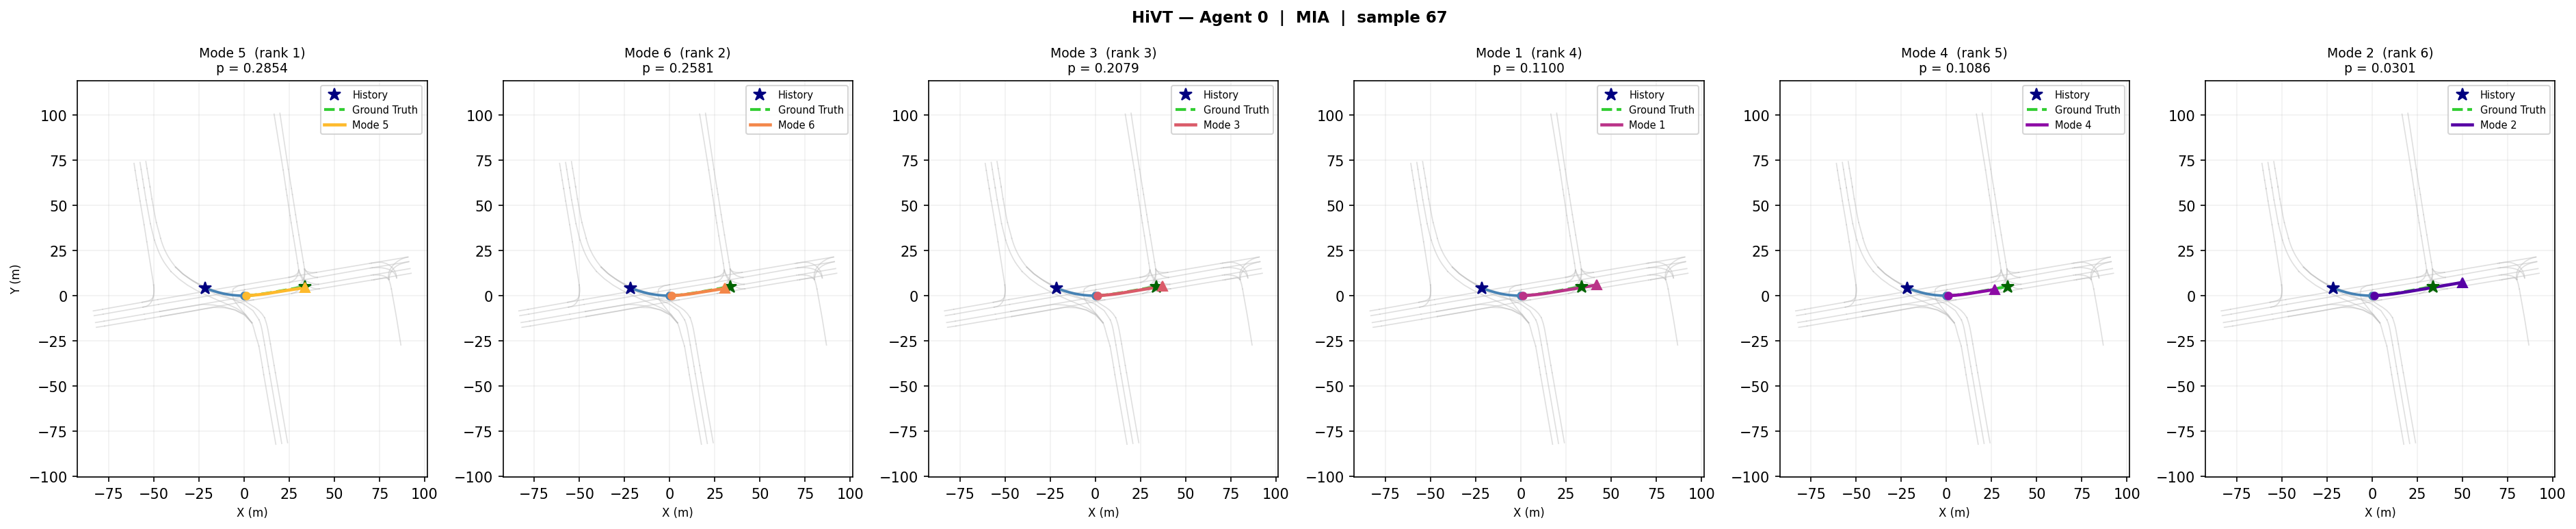
\includegraphics[width=\linewidth]{figures/traj_example.png}
  \caption{Qualitative prediction: the $K{=}6$ ranked modes for a focal agent at an
    intersection (star = history endpoint, green = ground truth, coloured =
    predicted mode), illustrating the multimodal output the distillation transfers.}
  \label{fig:traj}
\end{figure}

\paragraph{The calibration mechanism, directly.}
The diagnostics already embedded in the results sections isolate \emph{why} v1 fails
and v2 succeeds. Across the v1 $\lambda$-sweep the mode-weight entropy is flat while
the mean scale $b$ falls monotonically (Figure~\ref{fig:lambda32}); under v2 the
scale instead returns to the student's calibrated width (Table~\ref{tab:v2_32}).
The over-confidence therefore lives entirely in the per-mode scales, not in the
mixture weights---precisely the prediction of Section~\ref{ssec:method_calib}, and
the reason a distribution-matching target (which scores the teacher's spread, not
just its mean) is the correct fix.

\paragraph{Mode diversity.}
The students retain genuine multimodality rather than collapsing onto a single mode
under distillation: mode-weight entropy is preserved (above) and an offline
mode-diversity measurement confirms the predicted modes remain geometrically
distinct. This rules out the most common distillation failure---a student that
mimics only the teacher's dominant mode---and complements the permutation analysis
of Section~\ref{ssec:method_perm}, which established that the teacher and student
modes are mutually unaligned in the first place.
% TODO(optional): if a mode-diversity figure/number is wanted, generate it with
% visualisation_other_tests/measure_mode_diversity.py and cite the value here.
